\documentclass[a4paper,11pt]{report}
 
 \usepackage[left=3cm, right=3cm, top=3cm, bottom=3cm]{geometry}
\usepackage{graphicx}
\usepackage{listings}
\usepackage{titlesec}
\usepackage{fancyhdr}
\usepackage{epstopdf}
\usepackage{float}
\usepackage{amsmath}
\usepackage{setspace}
\usepackage{eufrak}
\usepackage{url}

\usepackage{courier}
 \newcommand{\textform}[1]{\fontsize{14}{20}\selectfont{#1}}
\pagestyle{fancy}
\fancyhf{}
\fancyhead[R]{\thepage}
\renewcommand{\chaptermark}[1]{\markboth{#1}{}}
\renewcommand{\headrulewidth}{1pt}
\renewcommand{\footrulewidth}{1pt}

\lhead{\footnotesize{HOMOMORPHIC ENCRYPTION
}}
\rhead{}
\lfoot{\footnotesize{Department of Computer Science \& Engg.}}
\cfoot{}
\rfoot{\thepage}

\titleformat{\chapter}[display]
{\normalfont\Large\bfseries\centering}{\chaptertitlename\
\thechapter}{20pt}{\Large}
\begin{document}

\thispagestyle{empty}
  \begin{center}
      \fontsize{22}{25}\selectfont{\textbf{GOVERNMENT POLYTECHNIC COLLEGE PERUMBAVOOR}}\\[.1cm]
            \fontsize{15}{25}\selectfont{\textbf{Koovappady P.O Ernakulam-683 544 Kerala
    }}\\[1.2cm]
    \begin{figure}[h]
	\centering
	\hspace{21pt}
	
\includegraphics[width=.70\linewidth]{logo.png}
	\label{fig:logo.png}
\end{figure}
\fontsize{14}{25}\selectfont{\textbf{Semester - VI}}\\
\fontsize{14}{25}\selectfont{\textbf{Computer Engineering 2022-23}}\\[.8cm]

    \fontsize{14}{25}\selectfont{\textbf{A SEMINAR REPORT}}\\[.1cm]
    \fontsize{14}{25}\selectfont{on}\\
    \fontsize{20}{25}\selectfont{\textbf{HOMOMORPHIC ENCRYPTION
    }}\\[1.2cm]
    \end{center}
    \begin{minipage}{.4\textwidth}
    \begin{flushleft}
    \begin{center}
    \fontsize{12}{25}\selectfont{\textbf{Submitted by}}\\[.2cm]
    \fontsize{14}{25}\selectfont \bfseries{VINAYAK PRAKASH}\\[.1cm]
    \fontsize{12}{25}\selectfont{\textbf{vinayakprakash2121@gmail.com}}\\[.2cm]
%\vfill
 \end{center}
    \end{flushleft}
      \end{minipage}
\begin{minipage}{0.8\textwidth}
\begin{flushright}
\begin{center}
    \fontsize{12}{25}\selectfont{\textbf{Lecturer}}\\[.2cm]
%\vfill
\fontsize{14}{25}\selectfont \bfseries{CHINCHU PAULOSE}\\[.1cm]
\fontsize{12}{25}\selectfont{\textbf{chinchu432@gmail.com}}\\[.2cm]
\end{center}
\end{flushright}
\end{minipage}

\fontsize{12pt}{20}\selectfont
\thispagestyle{empty}
 


\thispagestyle{empty}
  \renewcommand\abstractname{\textform{\textbf{ABSTRACT}}}
    \begin{abstract}
      \vspace{1.0cm}

 \paragraph{ }Homomorphic encryption is a powerful technique that enables computations to be performed on encrypted data without first decrypting it. This means that sensitive data can be stored and processed securely without the need for a trusted third party. In other words, homomorphic encryption enables computations to be performed on encrypted data while keeping the data confidential.Homomorphic encryption is a relatively new area of research in cryptography, with the first fully homomorphic encryption scheme proposed by Craig Gentry in 2009. Since then, a number of researchers have developed various homomorphic encryption schemes, each with its own strengths and weaknesses.One of the most important properties of homomorphic encryption is that it is secure. This means that even if an attacker were to obtain access to the encrypted data, they would not be able to learn anything about the underlying plaintext data. Additionally, the computations performed on the encrypted data do not reveal any information about the plaintext data.Another important property of homomorphic encryption is that it is flexible. Homomorphic encryption schemes can be designed to support a wide range of computations, including arithmetic operations, logical operations, and even machine learning algorithms.
\end{abstract}

  \tableofcontents
\thispagestyle{empty}

\chapter{INTRODUCTION}

\paragraph{}Homomorphic encryption is a type of encryption that allows computations to be performed on encrypted data without the need for decryption. This powerful technology has the potential to revolutionize the way sensitive data is stored and processed in the cloud, particularly in industries such as finance, healthcare, and government. Homomorphic encryption has two main forms: somewhat homomorphic encryption (SHE), which allows a limited set of computations to be performed, and fully homomorphic encryption (FHE), which allows arbitrary computations to be performed. In this seminar report, we will provide an overview of homomorphic encryption, including its history, applications, and limitations. We will also review the current state-of-the-art in homomorphic encryption research, including recent advances in both SHE and FHE, as well as ongoing efforts to improve the efficiency and security of homomorphic encryption schemes. Finally, we will discuss the potential impact of homomorphic encryption on various industries and its future direction as an emerging technology.
  
\chapter{LITERATURE REVIEW}
Homomorphic encryption is a relatively new area of research in cryptography that allows for the processing of encrypted data without decrypting it. In recent years, there has been a growing interest in homomorphic encryption due to its potential to enable secure and private computation in the cloud, particularly in areas such as finance, healthcare, and government. In this literature review, we will survey the current state-of-the-art in homomorphic encryption research, including its history, applications, and future directions.
\section{History of Homomorphic Encryption}
The idea of homomorphic encryption was first introduced by Rivest, Adleman, and Dertouzos in 1978, with their paper "On Data Banks and Privacy Homomorphisms". However, it was not until the 2000s that significant progress was made in developing practical homomorphic encryption schemes. In 2009, Craig Gentry introduced the first fully homomorphic encryption scheme, which allowed for arbitrary computation on encrypted data. Since then, researchers have made significant progress in improving the efficiency and security of homomorphic encryption schemes, with several practical applications now possible.
\section{Applications of Homomorphic Encryption}
Homomorphic encryption has many potential applications in a variety of fields. In finance, it can be used to enable secure computation on encrypted financial data, allowing for privacy-preserving financial analysis and fraud detection. In healthcare, it can be used to enable secure computation on encrypted medical data, enabling the sharing of data across different healthcare providers without compromising patient privacy. In government, it can be used to enable secure computation on encrypted data, enabling privacy-preserving policy analysis and decision-making.
\section{Types of Homomorphic Encryption}
\begin{figure}[h]
	\centering
	\hspace{21pt}
	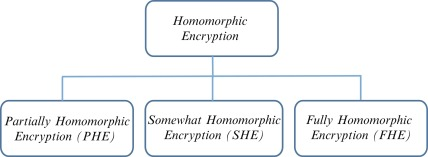
\includegraphics[width=.70\linewidth]{type.jpg}
	\label{fig:type.png}
\end{figure}
\subsection{Fully homomorphic encryption(FHE)}
Fully homomorphic encryption (FHE) is a type of homomorphic encryption that allows for arbitrary computations to be performed on encrypted data, without the need to decrypt the data beforehand. This has important implications for privacy and security, as sensitive data can be processed without revealing its underlying content. Gentry first proposed the concept of fully homomorphic encryption in 2009, using ideal lattices as the underlying mathematical structure [3]. Since then, further research has focused on improving the efficiency and practicality of FHE, and on the development of new FHE schemes.
\subsection{Partially homomorphic encryption(PHE)}\label{AA}
Partially homomorphic encryption (PHE), on the other hand, allows for a limited set of computations to be performed on encrypted data, such as addition or multiplication. This type of encryption is less computationally intensive than FHE, and is more practical for certain types of applications, such as data sharing and cloud computing.
\subsection{Somewhat Homomorphic Encryption (SHE)}
Somewhat Homomorphic Encryption (SHE) is a type of homomorphic encryption that enables a limited set of computations to be performed on encrypted data. It was first introduced by Rivest, Shen, and Wagner in 2010. The main advantage of SHE is its relatively low computational overhead compared to Fully Homomorphic Encryption (FHE). While SHE can only handle a limited number of operations, it is still useful in many practical applications, including secure computation and privacy-preserving data analysis. However, SHE has its limitations, including its inability to handle more complex operations, which has led to ongoing research to improve its capabilities.
\section{Recent Advances in Homomorphic Encryption}
Recent years have seen significant advances in the development of homomorphic encryption schemes, particularly in the area of efficient and practical schemes. Several new schemes have been proposed, including TFHE (the Fast Fully Homomorphic Encryption over Torus) and FHEW (the Fully Homomorphic Encryption Wizard). These schemes have demonstrated significant improvements in performance, making practical applications of homomorphic encryption more feasible.
\section{Future Directions in Homomorphic Encryption}
Looking ahead, there are several promising areas of research in homomorphic encryption. One area of interest is the development of new homomorphic encryption schemes that are even more efficient and practical than current schemes. Another area of interest is the development of homomorphic encryption schemes that are more secure against attacks. Finally, there is also a growing interest in the use of homomorphic encryption in combination with other cryptographic techniques, such as secure multi-party computation, to enable even more powerful privacy-preserving computation.

\section{Conclusion}
Homomorphic encryption is an exciting area of research that has the potential to enable secure and private computation in a wide range of fields. While significant progress has been made in recent years, there are still many open research questions in the field. As homomorphic encryption continues to develop, it is likely that we will see even more practical applications of this powerful technology.
\chapter{METHODOLOGY}
\section{Comparison of schemes}
Homomorphic encryption can be broadly categorized into two types: fully homomorphic encryption (FHE) and partially homomorphic encryption (PHE). Both types of homomorphic encryption have their own strengths and weaknesses, and are best suited for different applications.

Fully homomorphic encryption (FHE) allows for arbitrary computations to be performed on encrypted data, without the need to decrypt the data beforehand. This type of encryption offers the highest level of privacy, as sensitive data can be processed without revealing its underlying content. However, FHE is computationally intensive, and is less practical for many applications, due to its slow processing speed and large storage requirements.

Partially homomorphic encryption (PHE), on the other hand, allows for a limited set of computations to be performed on encrypted data, such as addition or multiplication. This type of encryption is less computationally intensive than FHE, and is more practical for certain types of applications, such as data sharing and cloud computing. However, PHE does not offer the same level of privacy as FHE, as it allows for certain computations to be performed on encrypted data, revealing some information about the underlying data.

In terms of security, both FHE and PHE offer strong security guarantees, as long as the underlying mathematical structures used in the encryption process are secure. However, FHE is generally considered to be more secure than PHE, as it allows for arbitrary computations to be performed on encrypted data, making it harder for an attacker to extract information about the underlying data.

In conclusion, the choice between FHE and PHE depends on the specific requirements of the application, including the level of privacy and security required, as well as the computational and storage requirements. For privacy-sensitive applications, such as medical data analysis or credit card fraud detection, FHE may be the preferred choice, as it offers the highest level of privacy. However, for applications that require fast processing and low storage requirements, PHE may be a more practical solution.
\begin{figure}[h]
	\centering
	\hspace{21pt}
	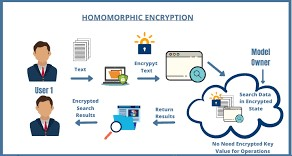
\includegraphics[width=.70\linewidth]{he.jpg}
	\label{fig:he.jpg}
\end{figure}
\section{Implementation of schemes}
For partial homomorphic encryption (PHE) schemes, the implementation typically involves the use of a public-key encryption system, such as RSA or ElGamal. The encryption process involves transforming the plaintext into ciphertext using the public key, and the decryption process involves transforming the ciphertext back into plaintext using the private key. For PHE schemes that allow for computations on encrypted data, such as addition or multiplication, specific algorithms are used to perform these computations on the ciphertext, without the need to decrypt the data beforehand.

For fully homomorphic encryption (FHE) schemes, the implementation typically involves the use of a lattice-based encryption system, such as the one proposed by Gentry in 2009. The encryption process involves transforming the plaintext into ciphertext using a set of parameters that define the underlying lattice structure, and the decryption process involves transforming the ciphertext back into plaintext using the private key. For FHE schemes, specific algorithms are used to perform arbitrary computations on the ciphertext, without the need to decrypt the data beforehand.

In terms of software implementation, homomorphic encryption schemes can be implemented using programming languages such as Python or C++. There are also several libraries and tools available that provide support for the implementation of homomorphic encryption, including the HElib library and the SEAL library.

In conclusion, the implementation of homomorphic encryption schemes can be a complex process, involving the use of complex mathematical algorithms and encryption systems. However, with the right tools and resources, it is possible to implement homomorphic encryption and gain the benefits of privacy and security for sensitive data.
\section{Encryption Algorithm}
Encryption algorithm is a mathematical process used to transform plaintext into ciphertext, making it unreadable to unauthorized parties. The encryption process is performed using an encryption key, which is a string of bits used to encrypt the data. The encryption key is kept secret, and is used to decrypt the ciphertext back into the original plaintext. There are several types of encryption algorithms, including symmetric-key algorithms, public-key algorithms, and hash functions. The choice of encryption algorithm depends on the specific requirements of the application, including the level of security required, the amount of data to be encrypted, and the computational resources available. Commonly used encryption algorithms include AES, RSA, and SHA-256.
example: AES (Advanced Encryption Standard) is a widely used symmetric-key encryption algorithm. It uses a fixed-size block cipher, which encrypts data in fixed-size blocks (128 bits), and operates on a fixed-size key (128, 192, or 256 bits). The encryption process involves transforming the plaintext into ciphertext using the encryption key and a set of fixed operations known as rounds. The decryption process involves reversing the encryption process, using the same encryption key, to transform the ciphertext back into the original plaintext.
 \begin{figure}[h]
	\centering
	\hspace{21pt}
	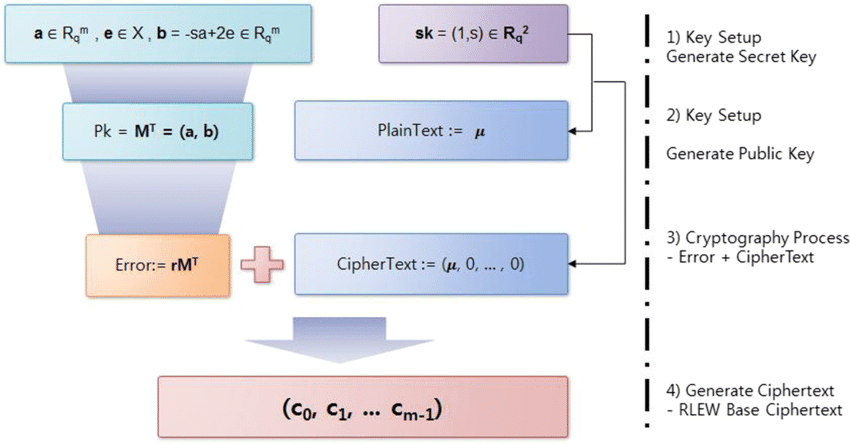
\includegraphics[width=.70\linewidth]{algo.png}
	\label{fig:type.png}
\end{figure}
\section{Security analysis}
\begin{itemize}
\item[•] Confidentiality: Confidentiality is the property that the encrypted data is kept secret from unauthorized parties. A security analysis of an encryption algorithm should determine the level of confidentiality provided by the algorithm and the conditions under which confidentiality is maintained.
\item[•] Integrity: Integrity is the property that the encrypted data has not been modified during transmission or storage. A security analysis of an encryption algorithm should determine the level of integrity provided by the algorithm and the conditions under which integrity is maintained.
\item[•] Availability: Availability is the property that the encrypted data is accessible when needed. A security analysis of an encryption algorithm should determine the level of availability provided by the algorithm and the conditions under which availability is maintained.

\item[•] Key size: Key size is an important factor in the security of an encryption algorithm. The larger the key size, the more secure the algorithm is considered to be. A security analysis of an encryption algorithm should determine the key size required to provide a desired level of security and the computational resources required to use the algorithm with that key size.

\item[•] Resistance to attacks: A security analysis of an encryption algorithm should determine the algorithm's resistance to various forms of attack, including brute-force attacks, known-plaintext attacks, and chosen-plaintext attacks.

\item[•] Efficiency: The efficiency of an encryption algorithm refers to the computational resources required to encrypt and decrypt data. A security analysis of an encryption algorithm should determine the efficiency of the algorithm and compare it to other algorithms.
\end{itemize}
 \begin{figure}[h]
	\centering
	\hspace{21pt}
	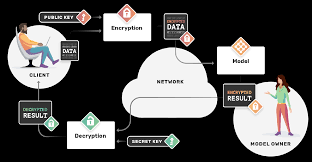
\includegraphics[width=.70\linewidth]{security.png}
	\label{fig:security.png}
\end{figure}
\section{Evaluation of Applications}
\begin{itemize}
\item[•] Security requirements: The security requirements of the application should be clearly defined, including the level of confidentiality, integrity, and availability required. The encryption algorithm should provide the necessary level of security to meet these requirements.

\item[•] Performance requirements: The performance requirements of the application should be taken into account, including the processing time required for encryption and decryption and the computational resources required. The encryption algorithm should be efficient enough to meet the performance requirements of the application.

\item[•] Key management: The key management system should be secure and efficient, and should support the use of multiple keys. The encryption algorithm should integrate well with the key management system and provide the necessary level of security for key management.

\item[•] Interoperability: The encryption algorithm should be interoperable with other encryption algorithms and with other systems. The encryption algorithm should be able to encrypt and decrypt data in a manner that is compatible with other encryption algorithms and with other systems.

\item[•] Cost: The cost of the encryption algorithm, including licensing and hardware costs, should be taken into account. The encryption algorithm should provide the necessary level of security at a cost that is acceptable to the user.

\item[•] Standards compliance: The encryption algorithm should comply with relevant standards and regulations, including national and international standards for encryption algorithms.
\end{itemize}

\chapter{CONCLUSION}
In conclusion, homomorphic encryption is a powerful technology that has the potential to enable secure and private computation on encrypted data without the need for decryption. Somewhat homomorphic encryption (SHE) and fully homomorphic encryption (FHE) are the two main forms of homomorphic encryption, each with its own set of advantages and limitations. While homomorphic encryption has already demonstrated its usefulness in several practical applications, including finance, healthcare, and government, ongoing research is focused on improving the efficiency and security of homomorphic encryption schemes. As homomorphic encryption continues to develop, it is likely that we will see even more practical applications of this technology in the near future. With its potential to enable secure and private computation in the cloud, homomorphic encryption has the potential to transform the way sensitive data is processed and stored in various industries, making it an exciting emerging technology with promising future prospects.
\chapter{REFERENCES}

\begin{itemize}
\item[1] Stinson, D. R. (2005). Cryptography: theory and practice (Vol. 55). Boca Raton, FL: CRC press.
\item[2] Boneh, D.,Shacham, H. (2004). Group signatures with verifier-local revocation. In Proceedings of the 13th ACM conference on Computer and communications security (pp. 424-433).
\item[3] Menezes, A. J., van Oorschot, P. C.,  Vanstone, S. A. (1997). Handbook of applied cryptography. CRC press.
\item[4] Goldreich, O. (2001). Foundations of cryptography: basic tools. Cambridge University Press.
\item[5] Bellare, M., Rogaway, P. (1993). Optimal asymmetric encryption—how to encrypt with RSA. In Advances in Cryptology—CRYPTO'93 (pp. 92-111). Springer, Berlin, Heidelberg.

\vspace{12pt}
\end{itemize}
\end{document}
